\documentclass[
  utf8,%     More capable input encoding than latin-1.
  % parskip,%  For vertical whitespace between paragraphs.  This comes down to more than just using parskip.sty, so it's better to use this class option.
  % S5MP % If you intend to really use margin paragraphs (not recommended!).
%  crop,%     Produce output with crop marks and paper size A4.  Liu-Tryck should like this.  Automatically adds information, including the physical page number, at the top of each page.
       %     Add option 'noInfo' to suppress the info at the top of each page when using option 'crop'.
  % Font options: 'kp' (default), 'times', 'lm'.  The KpFonts (loaded using 'kp'), is the most complete font among the provided options.  Among other, it supports slanted small caps.  See rtthesis.cls for more details regarding the font options.
  largesmallcaps,intlimits,widermath,% Good options to KpFonts.
  sharecounter,nobreak,definition=marks,%  See comments in the results chapter of this document for more information on these options!
  numbers, % If you want to cite references by numbers, use this option.
  noparts% Use option 'noparts' if you do not make use of part divisions.
]{rtthesis}

\usepackage{mythesis}

\begin{document}
\selectlanguage{english}

\frontmatter
\maketitle

\begin{abstract}[swedish]
  Det här som vi har hållit på med är jätteviktigt faktiskt och det vi gjort blev bara sååå bra.  Kanske inte helt otippat, men det glass är sååå gott!

Förresten har vi blivit bäst på att skriva rapporter, så nu ska ska vi inte gå in närmare på några detaljer såhär i sammanfattningen.

\end{abstract}

\begin{abstract}[english]
  Perception of depth, ego motion and robust keypoints is critical for SLAM and structure from motion applications. Neural networks have achieved great performance in perception tasks in recent years. But collecting labeled data for supervised training is labor intensive and costly. This thesis explores recent methods in unsupervised training of neural networks that can predict depth, ego motion, keypoints and do geometric consensus maximization. The benefit from unsupervised training is that the networks can learn from raw data collected from the camera sensor, as oppose to labeled data. The thesis focuses on training on images from a monocular camera, where no stereo or LIDAR data is available. The experiments compare different techniques for depth and ego motion prediction from previous research, and shows how the techniques can be combined successfully. A keypoint prediction network is evaluated and its performance is compared with the ORB detector provided by OpenCV. A geometric consensus network is also implemented and its performance is compared with the RANSAC algorithm in OpenCV. The consensus maximization network is trained on the output of the keypoint prediction network. For future work it is suggested that all networks could be combined and trained jointly to reach a better overall performance. The results show (1) which techniques in unsupervised depth prediction are most effective, (2) that the keypoint predicting network outperformed the ORB detector, and (3) that the consensus maximization network was able to classify outliers with comparable performance to the RANSAC algorithm of OpenCV.

\end{abstract}

\begin{acknowledgments}
  I would like to thank my supervisor Gustav Häger and examiner Per-Erik Forssén for their assistance and creative freedom letting me explore the topics that are of high interest to me. I would also like to thank the company Dyno Robotics for lending me the computer resources necessary to perform the experiments in this thesis.

  \addvspace{1em}
  \begin{flushright}
    \textit{%
      Linköping, October 2020\\
      Erik Örjehag%
    }
  \end{flushright}
\end{acknowledgments}


\tableofcontents
\begin{notation}% Passing the option "old" to the notation environment will redefine the notationtabular environment so that it produces an old style LaTeX tabular instead of a booktabs.sty style tabular.
  \centering

  \begin{notationtabular}{Math}{Notation}{Meaning}
    $\reals$ & The set of real numbers \\
    $m, M$ & Scalars are denoted in italics \\
    $\textbf{m}$ & Vector are denoted in lower case non-italics \\
    $\textbf{M}$ & Matrices are denoted in upper case non-italics \\
    $\textbf{m}_i$ & Row or column vector $i$ (depending on context) of matrix $\textbf{M}$\\
    $m_i$ & Element $i$ of vector $\mathrm{m}$\\
    $m_{ij}$ & Element at row $i$ and column $j$ of matrix $\mathrm{M}$ \\
    $[m_{ij}]_{M\times N}$ & Size of matrix can be denoted with a subscript.\\
    $\textbf{M}_{\mathrm{name}}$ & Subscripts can be used to give a unique name. \\
    $\textbf{M}^{\mathrm{name}}$ & Superscript can also be used for the same purpose. \\
    $\delta_x \textbf{I}$ & Discrete derivative with respect to $x$-axis of matrix $\textbf{I}$\\
    $\textbf{M}^T, \textbf{m}^T$ & Matrix or vector transpose\\
    $|m|$ & Absolute value of $m$\\
    $||\textbf{m}||$ & Length of vector $\textbf{m}$\\
    $\textbf{m}\cdot \textbf{m}$ & Vector dot product\\
  \end{notationtabular}

  \begin{notationtabular}{Abbreviations}{Abbreviation}{Meaning}
	\abbrSFM\index{SFM@\abbrSFM!abbreviation} & Structure From Motion\\    \abbrCNN\index{CNN@\abbrCNN!abbreviation} & Convolutional Neural Network\\ \abbrSSIM\index{SSIM@\abbrSSIM!abbreviation} & Structural Similarity index \cite{ssim}\\ \abbrRGB\index{RGB@\abbrRGB!abbreviation} & Red Green Blue, color space\\ \abbrRANSAC\index{RANSAC@\abbrRANSAC!abbreviation} & Random Sample Consensus \cite{ransac}\\
	\abbrSVD\index{SVD@\abbrSVD!abbreviation} & Singular Value Decomposition\\
  \end{notationtabular}
\end{notation}


\mainmatter
\chapter{Introduction}\label{cha:intro}

This thesis aims to show how new neural network techniques can be used to predict depth and relative camera motion for an image sequence captured by a monocular \abbrRGB camera. Imagine closing one eye and looking out into the world, it is trivial as a human to detect motion and estimate how the head moves in relation to what is seen. Calculating camera movement from an image sequence is a well studied problem and is usually done by finding corresponding features in the images and calculate (using projective geometry) which camera movement can give rise to such correspondences and their relative movement between frames in a sequence.

Recent research has shown that its possible to predict depth and relative motion from a sequence of images taken with a monocular \abbrRGB camera. The training data is a sequence of unlabeled images with a small relative motion, for example looking out from the front window of a moving car. Given a target view and a new nearby view its possible to train a depth predicting and pose predicting \abbrCNN jointly using a combined loss function. The depth and pose predictions are used to warp nearby views to the target view and the loss is based on the similarity achieved after warping.

\section{Contributions}

A performance comparison of different techniques described in current research papers. Training and testing on new datasets.

\section{Motivation}

Localization by only using visual input is highly desirable in robotics applications due to the low hardware cost and power consumption of using cameras compared to, for example, 3D lidars. Obtaining labeled data can be a tedious task, that's why this thesis will focus on unsupervised learning on unlabeled data.

\section{Research Questions}

\begin{enumerate}
	
	\item What ideas from previous work can be combined and what is the performance gains if any?
	\item How well does previous methods work on new datasets not tested in the original papers? In what ways do the results break down?
	\item What alteration to previous loss functions can be made to improve results?
	\item How does the amount of training data affect the results? Can the performance of the methods from previous research be improved simply by training on more data?
	\item Can the results from the original papers be replicated in the PyTorch framework?
	
\end{enumerate}

\section{Delimitations}

The visual localization problem can be solved using, for example, a stereoscopic camera or a time of flight camera. But this thesis will only explore the use of a monoscopic, non depth sensing, \abbrRGB camera, because it enables applications where hardware cost is a big factor.

In a full \abbrSFM pipeline both 3D-reconstruction, bundle adjustment and loop-closure detection is usually done as well. This will not be part of this thesis project.
\chapter{Background}\label{cha:background}

\section{Convolutional neural networks}

The central method used in this project is a deep learning algorithm called convolutional neural networks (\abbrCNN for short). A \abbrCNN architecture can successfully capture the spatial dependencies in an image through convolutional filtering operations with kernels of learnable weights and biases.

\begin{figure}[H]
	\centering
	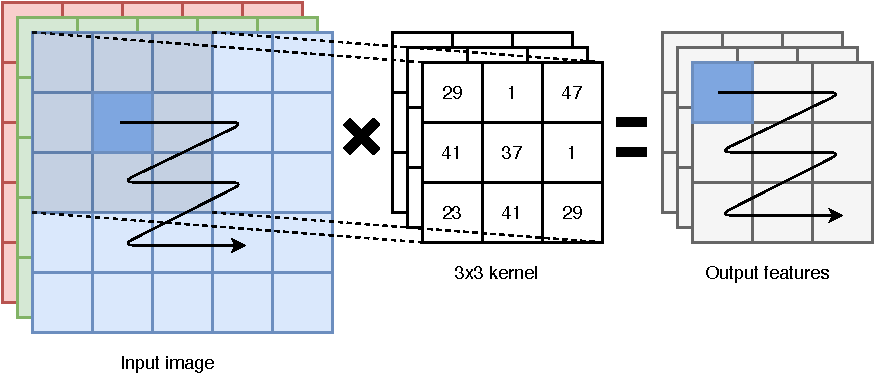
\includegraphics[width=0.9\textwidth]{conv}
	\caption{Convolutional filtering operation with a 3 channel RGB image and 3x3 kernel}
	\label{fig:conv}
\end{figure}

In Figure \ref{fig:conv} a convolutional filtering operation over an image is illustrated. The matrix kernel is moved in a row by row pattern and is multiplied by a patch of the image to get a value for the output cell.

In order to form a deep neural network multiple filtering operations are chained sequentially with nonlinear activation functions between them. A deep neural network usually consists of many such layers of filtering operations and activation functions. This concept is illustrated in Figure \ref{fig:deep}.

\begin{figure}[H]
	\centering
	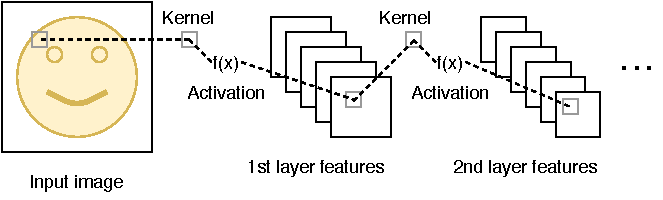
\includegraphics[width=0.8\textwidth]{deep}
	\caption{Multiple layers chained with each other to form a deep network}.
	\label{fig:deep}
\end{figure}

The activation functions need to be differentiable because the derivatives are used in the learning process. Some common nonlinear activation functions are shown in Figure \ref{fig:activation}.

\begin{figure}[H]
	\centering
	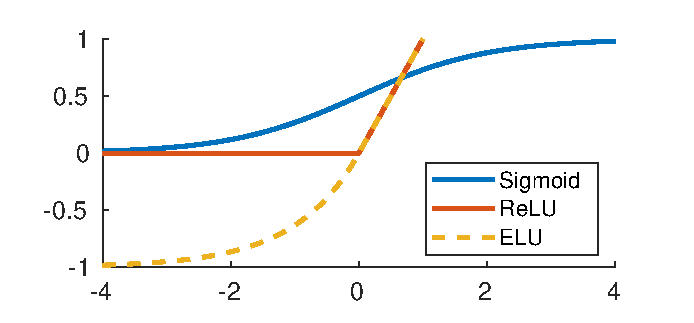
\includegraphics[width=0.6\textwidth]{activation}
	\caption{A few common nonlinear activation functions.}
	\label{fig:activation}
\end{figure}

The features in the deep neural networks are used to formulate a loss function. The loss defines an objective that we want the network to learn. This means that the process of learning becomes a task of updating the filter kernels in such a way that the loss function is minimized. If the loss function is decreasing during the training process it means that the network is learning. It is crucial that the loss function describes the problem accurately, otherwise the network will not learn the correct behavior. The weights in the network are updated using a method called back propagation. The algorithm computes the gradient of the loss function with respect to the weights in the network for a single input example from the training data using the derivative chain rule, which can be done very efficiently. Updating the weights to minimize the loss function can then be done using gradient decent. As the network is fed with more input examples from the training data, the network slowly learns the correct weights that minimizes the loss function as desired.





\section{Unsupervised learning}
\chapter{Related work}\label{cha:relatedwork}


In this chapter some of the important contributions of previous research papers are summarized. Firstly a list of papers in the field of unsupervised depth and ego motion prediction is presented. Secondly a paper on unsupervised feature point prediction. Thirdly a paper on unsupervised geometric consensus maximization that was implemented in this thesis. Finally a paper on combining depth and feature point prediction, albeit using classical consensus maximization that is not learned by a neural network.

\section{Unsupervised depth and ego motion prediction}
\label{sec:rldepth}

All the papers in this section are discussed in the order of publication to show a timeline of progress in the field of depth and ego motion prediction.

%\section{Unsupervised Monocular Depth Estimation with Left-Right Consistency}
%\label{sec:relwork:leftright}

In this paper\cite{leftright} the authors present MonoDepth, with an implementation available in Tensorflow on github. In this work the depth is predicted using an encoder-decoder type network, but the relative motion between frames is not estimated at all. The KITTI dataset provides stereo image pairs which are used during training, and the relative transformation between the left and right cameras is known. Using only the left image as input to the network both disparity maps for the left and right images are predicted. The two disparity maps are used to project the left image into the view of the right image and vice versa. This can be seen as a precursor to the papers discussed later which uses only a monocular camera and several frames over time to train a depth predicting network and pose predicting network jointly. The L1 norm of the per pixel photometric error as well as \abbrSSIM\cite{ssim} are computed and added to the loss. An additional loss term encourages the left disparity to be equal to the right disparity projected into the left camera viewpoint. Because the photometric error does not work well on low textured regions an edge aware smoothess term is added to propagate the depth values from nearby areas in the disparity map. The method produces metrically accurate results because the baseline and focal length of the cameras are known.

%\section{Unsupervised Learning of Depth and Ego-Motion from Video}
%\label{sec:relwork:unego}

In this paper\cite{sfmlearner} the authors present SfMLearner with an official implementation in Tensorflow on github. Contrary to the previous paper\cite{leftright} only a monocular sequence of images from the KITTI dataset is used during training. In the stereo case the relative pose between the left and right cameras was known, but with this monocular dataset the pose between subsequent frames is unknown. The authors train a pose predicting and depth predicting network simultaneously with a joint loss function to solve this problem. During training 3 subsequent frames are considered at a time. The frame $I_{t-1}$ and frame $I_{t+1}$ are called the source frames and the frame $I_t$ is called the target frame. The target frame is input to the depth network which estimates a disparity map. The two source frames are fed through a pose estimating network one after each other together with the target frame to find the relative transformations $T_{t	\rightarrow t-1}$ and $T_{t	\rightarrow t+1}$. The authors add an explainability mask to the photometric error term to account for errors in the model. The view synthesis formulation implicitly assumes that the scene does not contain moving objects, that there are no occlusions between the target and source frames, and that the surfaces are Lambertian so that the photo-consistency error of \abbrRGB values is meaningful. In order to predict the explainability mask an additional \abbrCNN is used. The network has no explicit supervisory signal but is encouraged to be non-zero with an regularization term using a cross-entropy loss with a constant label 1 at each pixel location. This makes the network minimize the view synthesis objective but is allowed some slack due to factors not considered by the model. In later work it was shown that the explainability mask does not help to improve results that much and is often ignored. To tackle the problem with textured areas and non Lambertian surfaces, a smoothess term is used. An edge aware smoothess term was not used like in previous work\cite{leftright} but a penalty on the second order gradient of the depth map was used instead. This unfortunately makes edges very fuzzy in the results compared to using the edge aware smoothness loss.

%\section{SuperDepth: Self-Supervised, Super-Resolved Monocular Depth Estimation}

% TA BORT?
In this paper\cite{superdepth} the authors train a depth estimating network on only stereo image pairs. After the depth predicting network has been trained the pose network from \cite{sfmlearner} is trained, using results from the already trained depth predicting network. This means that the depth and pose networks are not trained with a joint loss function but are instead trained separately. The main contributions from this paper is a new subpixel-convolution operation that super-resolve disparities from their low-resolution outputs, thereby replacing the up-sampling layers typically used in the disparity decoder network. The method additionally uses differentiable flip-augmentation to remove edge artifacts on the left and right edges of the depth map seen in previous work using stereo image pairs during training. To handle occluded pixels between the left and right images an occulsion regularization loss term is added to encourage background depths (low disparaty).

%\section{3D Packing for Self-Supervised Monocular Depth Estimation}

% TA BORT?
In this paper\cite{packnet} the authors present PacknetSfM. The main contribution is a new network architecture with packing and unpacking blocks replacing down and up sampling. The new packing blocks use space to depth transformations and 3d convolutions. The authors claim that the new packing and unpacking blocks are better at perserving resolution than standard down and upsampling. As the method is not adopted in later work, it is unclear if the new packing and unpacking approach is effective. The second contribution is a loss on the camera velocity that makes it possible for the monocular depth estimation to be metrically accurate. The velocity of the car is assumed to be known in the training dataset. The third contribution is a mask on pixels that do not change between frames. These pixels are assumed to be part of objects that are stationary with respect to the camera. Such pixels can occur for example if the car dashboard is visible in a frame, or other vehicles are moving at a similar speed nearby.

%\section{Digging Into Self-Supervised Monocular Depth Estimation}

In this paper\cite{monodepth2} the authors present MonoDepth2. They propose mainly two contributions. Firstly, instead of taking the average of the reprojection errors from all source frames given a target frame they use the minimum. This makes it so that if a feature is occluded in one source image but not in the other the errors will not be averaged together but instead the error from the source frame that is not occluded will be used. Secondly, instead of calculating the loss for each depth scale in the decoder, all the depth maps are up-sampled to the original target image size when computing the loss. This way a single pixel in the low resolution layer of the decoder will predict the depth of a patch of pixels in the originally sized input image.

\section{Unsupervised keypoint prediction}
%\section{UnsuperPoint: End-To-End Unsupervised Interest Point Detector and Descriptor}

Collecting ground truth data to train a neural network for keypoint detection is cumbersome. What constitutes a keypoint is hard to define clearly and consistently for a human annotator.

SuperPoint\cite{superpoint} uses a unsupervised approach to learn prediction of points and their descriptors. The network is first trained on  a synthetic dataset of simple geometric shapes. The pseudo ground truth points are defined as the corners and junctions in the synthetic images. This pre-trained network is then trained on "real" images in a siemese network setup using a method they call homographic adaptation. The two siamese siblings are fed images transformed by random but known homographies and the output from the networks are compared in the loss function. The output of SuperPoint is a heatmap where each pixel describes the "point-ness" of that pixel, and a descriptor map. To keep the model fast both the point and descriptor maps are predicted semi-dense grid,
one cell for each 8 pixel patch. The maps are up-sampled to the original image size using bicubic interpolation, and the descriptors are normalized.

UnsuperPoint\cite{unsuperpoint} is heavily inspired by SuperPoint but does not need to be pre-trained on a synthetic dataset, instead it is trained in one round of training on real images. It uses a similar method of using siamese networks and homography adaptation during traning, but the output from the network is different. The network uses regression of actual point position coordinates instead of a heat map, incorporates non-maximum suppression, predicts scores for each keypoint and a sparse descriptor map that is sampled and interpolated using the point positions.

\section{Unsupervised geometric consensus maximization}
%\section{Unsupervised Learning of Consensus Maximization for 3D Vision Problems}

Consensus maximization is an important strategy in 3D vision problems for robust geometric model estimation from measurements including outliers. The classical method of \textit{Random Sampling and Consensus}, or RANSAC\cite{ransac} for short, is widely popular with great success. But replicating the same generic behavior using supervised training of neural networks has proven difficult. Unsupervised methods have a huge potential to generalize to any unseen data distribution and are in this context very desirable. This paper\cite{consensus} introduces just such an unsupervised method of consensus maximization for 3D vision problems. Using the relationship between the set of inliers, and the subspace of polynomials representing the space of target transformations a model fitting cost can be can be defined without knowing the specific parameters of the geometric transformation. During learning the loss is defined in a way to learn the largest set of inliers with a low model fitting cost. The geometric model parameters can then be extracted from the polynomials after network has learnt to distinguish inliers and outliers.

\section{Combined depth and feature point detection}

In a paper\cite{keypointdepth} the authors combines the previously discussed MonoDepth2\cite{monodepth2} for depth prediction, but also adds keypoint learning from SuperPoint\cite{superpoint} into the pipeline. The researchers train the depth, keypoint and pose estimating networks jointly, making them benifit from each other and achieve state of the art performance.  However, the step that finds possible outlier keypoints, is not differentiable and is not trained jointy with the depth and keypoint networks. The step that calculates the model parameters of the geometric relationship between corresponding keypoints also requires an initial guess that is not differentiable.


\chapter{Method}\label{cha:method}

\section{Convolutional neural networks}

The central method used in this project is a deep learning algorithm called convolutional neural networks (\abbrCNN for short). A \abbrCNN architecture can successfully capture the spatial dependencies in an image through convolutional filtering operations with kernels of learnable weights and biases.

\begin{figure}[H]
	\centering
	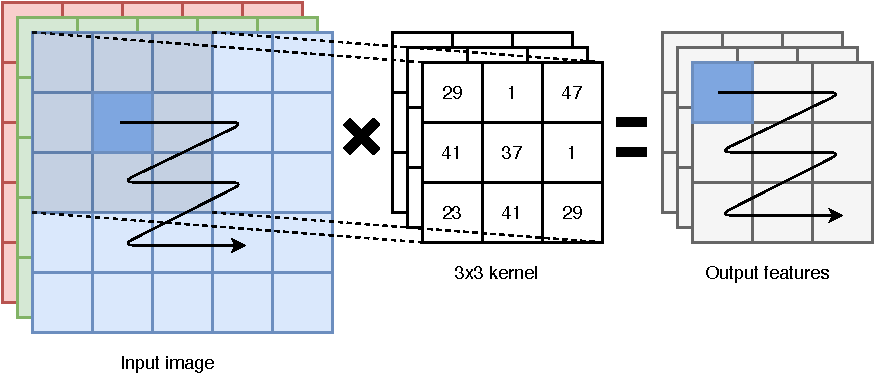
\includegraphics[width=0.9\textwidth]{conv}
	\caption{Convolutional filtering operation with a 3 channel RGB image and 3x3 kernel}
	\label{fig:conv}
\end{figure}

In Figure \ref{fig:conv} a convolutional filtering operation over an image is illustrated. The matrix kernel is moved in a row by row pattern and is multiplied by a patch of the image to get a value for the output cell.

In order to form a deep neural network multiple filtering operations are chained sequentially with nonlinear activation functions between them. A deep neural network usually consists of many such layers of filtering operations and activation functions. This concept is illustrated in Figure \ref{fig:deep}.

\begin{figure}[H]
	\centering
	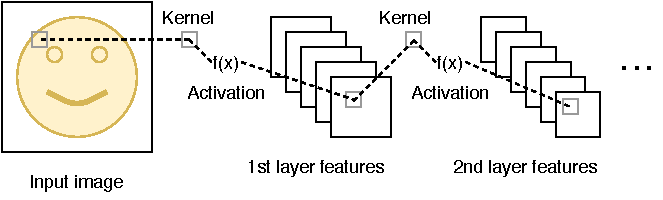
\includegraphics[width=0.8\textwidth]{deep}
	\caption{Multiple layers chained with each other to form a deep network}.
	\label{fig:deep}
\end{figure}

The activation functions need to be differentiable because the derivatives are used in the learning process. Some common nonlinear activation functions are shown in Figure \ref{fig:activation}.

\begin{figure}[H]
	\centering
	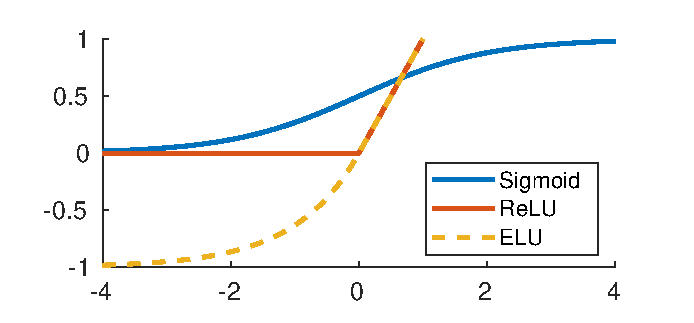
\includegraphics[width=0.6\textwidth]{activation}
	\caption{A few common nonlinear activation functions.}
	\label{fig:activation}
\end{figure}

The features in the deep neural networks are used to formulate a loss function. The loss defines an objective that we want the network to learn. This means that the process of learning becomes a task of updating the filter kernels in such a way that the loss function is minimized. If the loss function is decreasing during the training process it means that the network is learning. It is crucial that the loss function describes the problem accurately, otherwise the network will not learn the correct behavior. The weights in the network are updated using a method called back propagation. The algorithm computes the gradient of the loss function with respect to the weights in the network for a single input example from the training data using the derivative chain rule, which can be done very efficiently. Updating the weights to minimize the loss function can then be done using gradient decent. As the network is fed with more input examples from the training data, the network slowly learns the correct weights that minimizes the loss function as desired.





\section{Unsupervised learning}

\section{Datasets}

The neural networks are trained and evaluated on images from 2 different datasets, KITTI\cite{kitti} and Lyft\cite{lyft2019}. Both datasets are preprocessed to remove frames where the camera is not moving. This is important because if there is no movement between frames then no depth information can be inferred during training when using monoscopic data. In the Kitti dataset the images from the left and right camera are treated as separate image sequences to yield more training data. The images are resized to $128\times 416$ pixels, and the intrinsic camera matrix is updated accordingly.

\subsection{Sequence datasets}

To train the networks used for depth and ego motion prediction the images from Kitti and Lyft at loaded in triplets of subsequent frames in a sequence.

The lidar data from Kitti and Lyft is converted to a sparse depth map, together with the ground truth ego motion. This data is only used during testing, not during training.
adjacent
\begin{figure}[H]
	\centering
	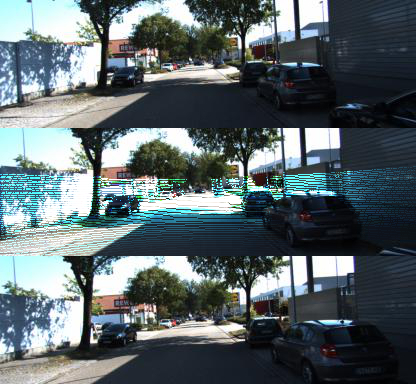
\includegraphics[width=0.5\textwidth]{sequencedataset}
	\caption{The dataloader loads 3 subsequent frames in a sequence. The figure shows from top to bottom 3 frames from Kitti, $I_{t-1}$, $I_t$, $I_{t+1}$ with the sparse depth map overlayed on frame $I_t$.}
	\label{fig:sequencedataset}
\end{figure}

Kitti contains 124 sequences, and Lyft contains 148 sequences. For each dataset the sequences are split, approximately 90\% is used for training and 10\% for testing.

\begin{table}[H]
	\centering
	\begin{tabular}{ |c|c|c|c|c| } 
		\hline
		&\multicolumn{2}{c|}{Sequences / Samples} \\ 
		\hline
		& Train & Test \\ 
		\hline
		Kitti & 110 / 16542 & 12 / 11349 \\ 
		\hline
		Lyft & 134 / 3759 & 14 / 1735 \\ 
		\hline
	\end{tabular}
	\caption{The training sequences are split into a training set and a testing set.}
	\label{table:datasets}
\end{table}

\subsection{Homographic adaptation dataset}

To train the network that predicts keypoints, images are read one by one from the Kitti or Lyft datasets. The image is fed trough two branches, in branch A the image is not modified, and in branch B the image is transformed by a random homography (Figure \ref{fig:unsuperpointloss}). The authors of UnsuperPoint refer to this technique as homographic adaptation.

How to generate the random homography used during training is not described in the UnsuperPoint paper, but is an important part of the method. The method used in this thesis generates random homographies from 5 parameters $\alpha_{rotation}$, $\alpha_{translation}$, $\alpha_{scale}$, $\alpha_{sheer}$ and $\alpha_{perspective}$. The parameters controls the maximum transformation for each aspect of an homography. The final homographgy is constructed from parts as follows.

\[
H = H_{affine} H_{sheer} H_{perspective}
\]

Assume $u_n \sim U(-1,1)$ are random uniform variables in the range -1 to 1.

\[
H_{affine} = 
\begin{pmatrix}
\cos(r)*s & -\sin(r) & t_x \\
\sin(r)& \cos(r)*s & t_y \\
0 & 0 & 1 \\
\end{pmatrix}
, \text{with}
\begin{cases}
r=u_1*\alpha_{rotation} \\
s=u_2*\alpha_{scale}+1 \\
t_x=u_3*\alpha_{translation} \\
t_y=u_4*\alpha_{translation} \\
\end{cases}
\]

\[
H_{sheer} = 
\begin{pmatrix}
1 & s & 0 \\
s & 1 & 0 \\
0 & 0 & 1 \\
\end{pmatrix}
, \text{with}
\ s=u_5*\alpha_{sheer} \\
\]

\[
H_{perspective} = 
\begin{pmatrix}
1 & 0 & 0 \\
0 & 1 & 0 \\
p & p & 1 \\
\end{pmatrix}
, \text{with}
\ p=u_6*\alpha_{perspective} \\
\]

The output from the network is used together with the random but known homography to formulate the loss function.

TODO: Illustration of training data for consensus maximization


\section{Architectures}

In order to predict depth and motion from monocular images two different CNN architectures are examined.

\subsection{SfMLearner architecture}
This is the architecture from \cite{sfmlearner}. The authors use a DispNet\cite{dispnet} architecture to predict depth maps at four different scales, and a ResNet18\cite{resnet} architecture with modified decoder to predict pose updates in an euler angle axis representation.



\subsection{Monodepth2 architecture}
This is the architecture from \cite{monodepth2}. The authors use a ResNet18 architecture instead of a DispNet architecture to predict depth estimates. They make this choice because its a smaller and faster architecture. Similarly they use a ResNet18 architecture with modified decoder to predict the pose updates in an euler angle axis representation.



%\subsection{Data augmentation}

Following \cite{monodepth2} the ability to apply a random augmentation with 50\% chance to the training images will be implemented in the system. This can improve robustness and hopefully makes the CNN generalize and achieve better results on the unseen testing data. The following augmentations can be applied: Horizontal flip, random brightness, contrast, saturation and hue jitter.

\section{Differentiable depth image warping}
\label{sec:diffwarp}

Central to all previous methods in the related work section is the differentiable depth image warp operation in the loss function of the CNN networks. Given the intrinsic camera matrix:

\[
K = 
\begin{pmatrix}
f_x & s & x_0 \\
0 & f_y & y_0 \\
0 & 0   & 1
\end{pmatrix}
\]

And the predicted depth $ D_t(p_t) $ of pixel $ p_t $ of the target (current) frame. And the transform $ T_{t \rightarrow s} $ from the target to source (next/previous) frame:

\[
T_{t \rightarrow s} =
\begin{pmatrix}
\textbf{R} & \textbf{t} \\
0 & 1
\end{pmatrix}
\]

The position of the target pixel $ p_t $ in the source image $ p_s $ can be calculated in homogeneous coordinates as:

\[
p_s \sim K T_{t \rightarrow s} D_t(p_t) K^{-1} p_t 
\]

The pixel position $ p_s $ is however continuous and in order to sample the discrete source image $ I_s $ a differentiable bilinear sampling method is used. The method is described in \textit{spatial transformer networks}\cite{spatialtransformernetworks} and works by interpolating the neighbouring 4 pixels values (top-left, bottom-right) by the distance to the the continuous sampling point $ p_t $.


\begin{figure}[H]
	\centering
	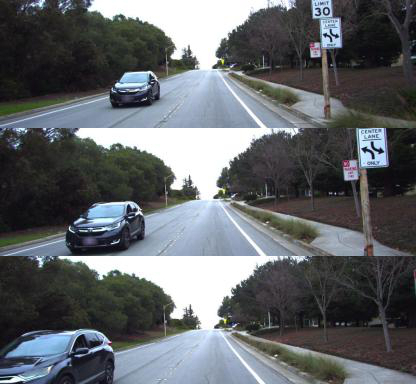
\includegraphics[width=0.6\textwidth]{seq}
	\caption{Sequence of images}
	\label{fig:sequence}
\end{figure}

\section{Loss functions}
\label{sec:loss}

\paragraph{Photometric loss} Is defined as $ \mathcal{L}_p(I_t, \hat{I}_s)=|I_t - \hat{I}_s| $.

\paragraph{SSIM loss} Is defined as $ \mathcal{L}_{ssim}(I_t, \hat{I}_s)=\dfrac{1-\textrm{SSIM}(I_t, \hat{I}_s)}{2} $.

\paragraph{Combined loss} The photometric and SSIM loss is often combined and balanced using $ \mathcal{L}_{ps}(I_t, \hat{I}_s) = \alpha \mathcal{L}_{ssim} + (1-\alpha) \mathcal{L}_p $

\paragraph{Depth smooth loss} Is defined as $ \mathcal{L}_{smooth}(D_t)=|\delta_x^2 D_t|+|\delta_y^2 D_t| $. Not ideal because it can cause very fussy edges as seen in SfMLearner.

\paragraph{Edge aware depth smooth loss} Is defined as $ \mathcal{L}_{edge}(D_t)=|\delta_x D_t|e^{-|\delta_x I_t|} + |\delta_y D_t|e^{-|\delta_y I_t|} $. Applied in Monodepth2 giving sharper edges because the smoothness term is weighted to mostly affect areas with small photometric derivitive.

\paragraph{Velocity supervision loss} When a velocity measurement exists in the dataset a term to enforce scale accurate estimates can be added like $ \mathcal{L}_{v} = \bigr{|} \| \textbf{t}_{t \rightarrow s} \| - |v|\Delta t \bigr{|} $, as proposed in packnet\cite{packnet}.

\subsection{Handling occlusions}
\label{sec:occlusion}

\paragraph{Disparity loss} To encourage background depths (low disparities) in shadows of the depth map where occlusion has occurred a penalty on the disparity can be added $ \mathcal{L}_{o} =|d_t|. $

\paragraph{Minimum loss across frames} In SfMLearner the photometric loss is calculated for the previous and next frames compared to the current in the sequence. The pixel wise average across the frames are then used. This causes problems if a pixel is for example occluded in the previous frame, but visible in the current and next frame. In this situation the average loss will be pretty high even though a correct depth and transformation has been predicted, because of the occluded pixel. Instead Monodepth2 suggests to pick the minimum per pixel error over the frames which creates a more telling loss. 


\section{Handling model limitations}
\label{sec:modellimit}

In order to optimize using the photometric reprojecton error as the loss function two assumptions must hold. Firstly the scene must be static, meaning all objects in the scene must be still except the moving camera. Movement by cars and humans in the scene that is not due to the camera movement will cause problems. Secondly there must be photometric consistency between frames for the photometric error to make sense. This means that non lambertian surfaces, change in lighting, and change in exposure between frames will cause problems.

\paragraph{Explainability mask} The authors of \cite{sfmlearner} tackle this problem by having a CNN predict what pixels are valid to use in the photometric loss function. It shares the encoder of the pose predicting network but branches of into a different encoder which estimates a mask of the valid/explainable pixels. The loss function for the mask is the cross entropy loss compared to a mask filled with ones. The photometric loss function is augmented to include the explainability mask removing pixels that cannot be explained by the predicted depth and transformation. This encourages the mask to be filled with ones, but allows some slack due to pixels that can not be explained by the photometric loss.

\paragraph{Stationary pixels mask} The authors of \cite{monodepth2} introduced a mask to remove stationary pixels from the set of previous, current and next frame. This is done by creating a mask where the photometric error is smaller before applying the projection than after. This works because stationary pixels that have not moved in relation to the camera will of course have a small photometric loss without reprojection. This will remove pixels from the car dashboard and also nearby vehicles that are traveling at the same speed.

\section{Handling model limitations}

\section{Evaluation metrics}

This section describes the metrics used to evaluate depth, ego motion, feature point and consensus maximization predictions. These specific metrics where chosen because they are also used in the related works in this field, which makes the results comparable to other papers.

\subsection{Depth error and accuracy metrics}
\label{sec:depthmetrics}

The depth error and accuracy metrics are sparse and only calculated for the pixels of which there exists a ground truth laser measurement in the dataset. The values are averaged over all laser measurements and frames in the test split of the dataset. An error of 0 and an accuracy of 1 is optimal, but can never be achieved in practice.

The depth is predicted relative to an unknown scale, and the ground truth is measured in meters. To alleviate this issue the depth predictions are scaled so that their median is the same as the median of the ground truth for each frame. This does not guarantee that the unit of the predictions is meters, but at least it makes the scales somewhat similar.

The error metrics used in the results chapter are referred to as \textit{Abs Rel}, \textit{Sq Rel}, \textit{RMSE} and \textit{RMSLE}.

The \textit{Abs Rel} error is based on \textit{MAE} which is the mean of the absolute errors which means that it has the same unit as the errors, and is conceptually quite easy to interpret.

\[
\textrm{MAE}=\frac{\sum^N_{n=1}{|y_n-\hat{y}_n|}}{N}
\]

Because the depth from the neural network is without unit and only predicted relative to an unknown scale, a variation on the \textit{MSE} metric called \textit{Abs Rel} is used.

\[
\textrm{Abs Rel}=\frac{\sum^N_{n=1}{\frac{|y_n-\hat{y}_n|}{y_n}}}{N}
\]

The \textit{MSE} metric is the mean of squared errors, for an unbiased estimator it represents the variance of the errors. 

\[
\textrm{MSE}=\frac{\sum^N_{n=1}{(y_n-\hat{y}_n)^2}}{N}
\]

Once again, because the depth is predicted relative to an unknown scale a variation on \textit{MSE} called \textit{Sq Rel} is used instead.

\[
\textrm{Sq Rel}=\frac{\sum^N_{n=1}{\frac{(y_n-\hat{y}_n)^2}{y_n}}}{N}
\]

The \textit{RMSE} metric is the square root of the mean of squared errors. For an unbiased estimator it represents the standard deviation of the errors. Because the errors are squared in the \textit{RMSE} metric it is more sensitive to outliers that for example \textit{MSE}.

\[
\textrm{RMSE}=\sqrt{\frac{\sum^N_{n=1}{(y_n-\hat{y}_n)^2}}{N}}
\]

The \textit{RMSLE} metric is similar to \textit{RMSE} but is useful because it penalizes large errors less when both the actual and predicted values are large.

\[
\textrm{RMSLE}=\sqrt{\frac{\sum^N_{n=1}{(\log{y_n}-\log{\hat{y}_n)}^2}}{N}}
\]

To measure the depth accuracy, in the range from 0 to 1, the following metric is used.

\[
a_{\gamma} = \frac{\sum^N_{n=1}{(\max(\frac{y_n}{\hat{y}_n}, \frac{\hat{y}_n}{y_n}) < \gamma)}}{N},\textrm{ for }\gamma \in \{1.25, 1.25^2, 1.25^3\}
\]

This should be interpreted as the ratio of predictions that is within the ratio of $ \gamma $ relative to the ground truth.

\subsection{Camera ego motion error metric}
\label{sec:egometric}

The error of the camera motion predictions are measured using \textit{RMSE}. But instead of taking the mean error over all poses in a sequence, the alignment error is calculated part wise over a track length of only 5 poses. The final error is presented as the mean \textit{RMSE} of all parts. Each track part from the prediction is transformed to have its first pose coincide with the ground truth in a common origo. This is done so that the first pose in the track part of both the prediction and ground truth is the identity matrix $I \in \mathbb{R}^{4\times 4}$. Because the ego motion is predicted relative to an unknown scale and the ground truth is in meters, we scale each predicted track part to have similar scale to the ground truth track part.

\subsection{Keypoint error and score metrics}\label{sec:keypointmetrics}

The unsupervised keypoint network was compared with the ORB feature detector from OpenCV. To messure the performance differences 3 different metrics where used, repeatability score (RS), localization error (LE), matching score (MS), and matching ratio (MR).

Before any of the metrics are calculated the points are first filtered to remove all points within 10px of the edges. This is done to not include detections where the black background meets the border of the transformed image.

\begin{figure}[H]
	\centering
	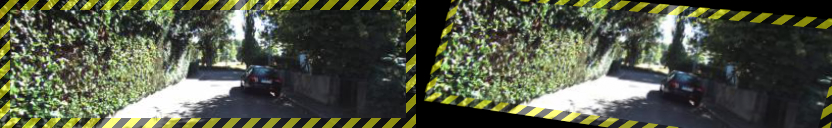
\includegraphics[width=1.0\textwidth]{remove-edges}
	\caption{The black and yellow stripes illustrates the are where keypoint detections are filtered out and discarded.}
	\label{fig:remove-edges}
\end{figure}

To calculate the set of ground truth correspondences, the points in the left image is transformed by the known homography $H$. A point in the left image is corresponding with a point in the right image if they are their closes neighbor and the distance is less than 3px after the transformation. This set of ground truth correspondences is used in all metrics. If the images contain a different amount of points, the largest set of possible correspondences that could have been found is $N_{tot} = \min(N_{left}, N_{right})$. The number of ground truth correspondences (closer than 3px) is $N_{gt} \le N_{tot}$.

Repeatability score (RS) is a measure on how good a method is at repeatedly highlighting the same physical features in the scene but in different images. Because the keypoint algorithm is only fed one image at the time, it is important that there is consistency in what physical features are selected in the image, otherwise their will be very few actual correspondences.

\[
RS = \frac{N_{gt}}{N_{tot}} 
\]

Localization error (LE) is a measure of the average distance error between the ground truth corresponding points. It will always be less than 3px because that is our definition of a correspondence, but the ideal is 0px.


Matching score (MS) is a measure on how many keypoints are matched correctly based on their descriptors. The set of points that are both ground truth correspondences and are corresponding based on their predicted descriptors are said to be correctly matched. The number of correctly matched points are $N_{correct}$.

\[
MS=\frac{N_{correct}}{N_{tot}}
\]

Matching ratio (MR) is very similar to matching score. To get a high MS requires both good repeatability and good descriptors, but getting an MR requires only good descriptors.

\[
MR=\frac{N_{correct}}{N_{gt}}
\]

\subsection{Consensus maximization performance metrics}\label{sec:consensusmetrics}

The unsupervised consensus maximization network that predicts homographies was compared with the \textit{findHomography()} function in OpenCV.

The homography error (HE) is calculated as the average distance between the corners of the image when it is transformed by the estimated homography compared to the ground truth homography.

\begin{figure}[H]
	\centering
	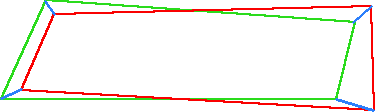
\includegraphics[width=0.5\textwidth]{he}
	\caption{The corners of the image transformed by the ground truth homography and the predicted homography is shown in green and red respectively. The homography error (HE) is calculated as the average of the distances shown in blue.}
	\label{fig:he}
\end{figure}

In order to evaluate the methods ability to distinguish inliers and outliers among the points, a confusion matrix is used. The ground truth set of inliers, or ideal, is the same as the one calculated in section \ref{sec:keypointmetrics}. The confusion matrix shows the ratio of true positives, true negatives, false positives and false negatives in the inlier classifications. The confusion matrix is normalized on the axis of ground truth so that the sum of true positives and false negatives adds up to 1, and the sum of the false positives and true negatives also adds up to one.

\begin{table}[H]
	\centering
	\begin{tabular}{l|l|c|c|c}
		\multicolumn{2}{c}{}&\multicolumn{2}{c}{Predicted}&\\
		\cline{3-4}
		\multicolumn{2}{c|}{}&Inlier&Outlier&\multicolumn{1}{c}{Total}\\
		\cline{2-4}
		\multirow{2}{*}{Actual}& Inlier & TP & FN & $TP+FN=1$\\
		\cline{2-4}
		& Outlier & FP & TN & $FP+TN=1$\\
		\cline{2-4}
		\multicolumn{1}{c}{} & \multicolumn{1}{c}{Total} & \multicolumn{1}{c}{$TP+FP$} & \multicolumn{    1}{c}{$FN+TN$} & \multicolumn{1}{c}{$2$}\\
	\end{tabular}
	\caption{Structure of confusion matrix for inlier classification.}
	\label{table:confusion}
\end{table}


\chapter{Resultat}\label{cha:Research}

Figure \ref{fig:evaluation} contains some preliminary evaluation results. The gray configurations in Figure \ref{fig:configurations} have not been trained yet. Each configuration takes about 15 hours to train. Still missing possibility to train on Synthia and also random data augmentations, L1 loss on disparity and velocity supervision loss.

\begin{figure}[H]
	\centering
	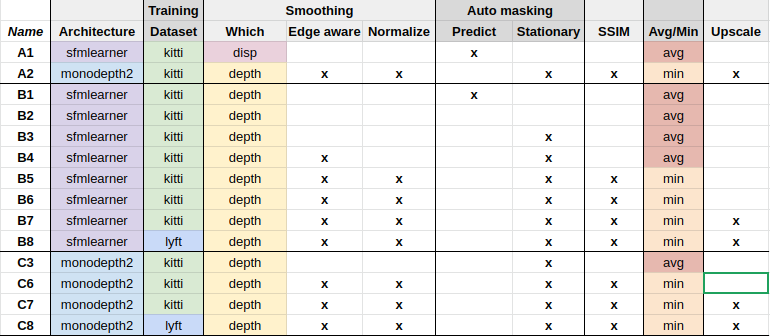
\includegraphics[width=1.0\textwidth]{configurations}
	\caption{Different configurations of network architecutes, training datasets and loss terms evaluated to find the best performance}
	\label{fig:configurations}
\end{figure}

\begin{figure}[H]
	\centering
	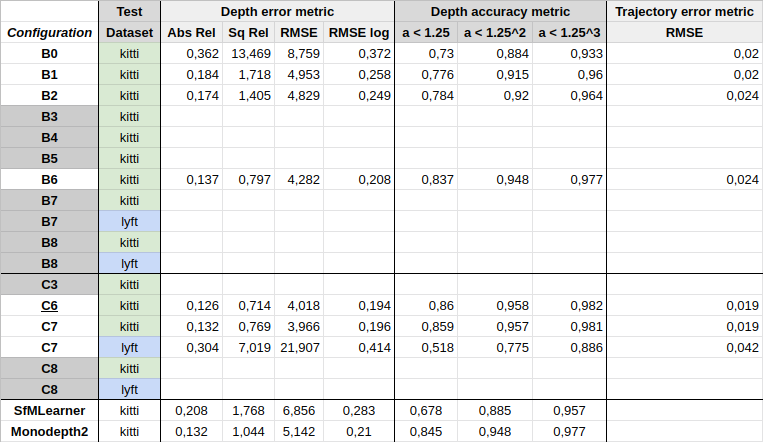
\includegraphics[width=1.0\textwidth]{evaluation}
	\caption{Evaluation metrics when testing the configurations on the testing split of the datasets}
	\label{fig:evaluation}
\end{figure}

\clearpage

\begin{figure}[H]
	\centering
	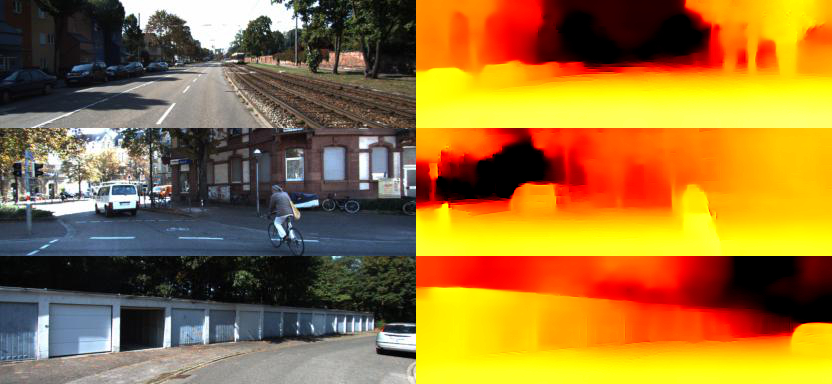
\includegraphics[width=1.0\textwidth]{depthmaps}
	\caption{Examples from the Kitti dataset}
	\label{fig:depthmapskitty}
\end{figure}

%\begin{figure}[H]
%	\centering
%	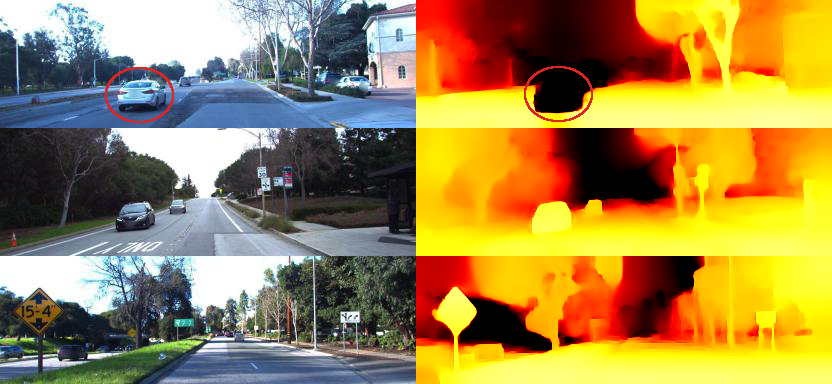
\includegraphics[width=1.0\textwidth]{depthmapslyft}
%	\caption{Examples from the Lyft dataset}
%	\label{fig:depthmaplyft}
%\end{figure}

\begin{figure}[H]
	\centering
	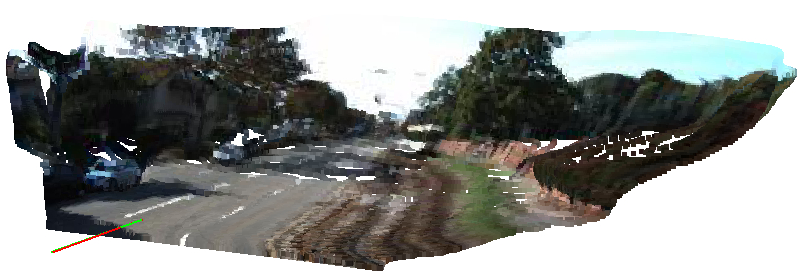
\includegraphics[width=0.8\textwidth]{3drender}
	\caption{3D render of colorized depth map}
	\label{fig:3drender}
\end{figure}

\begin{figure}[H]
	\centering
	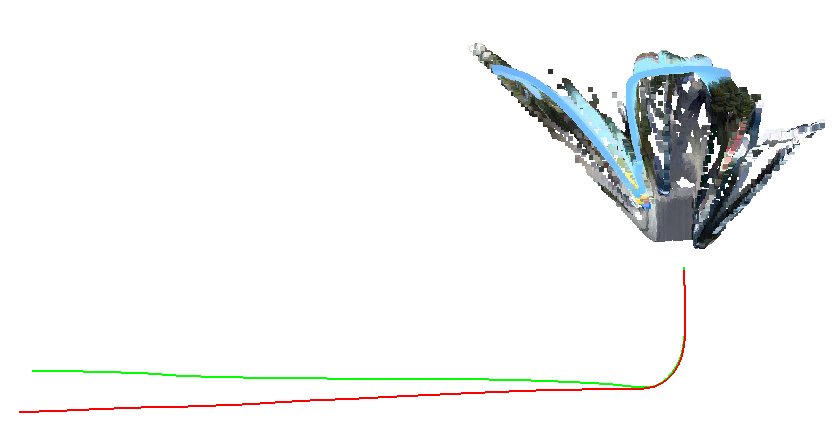
\includegraphics[width=0.8\textwidth]{movement}
	\caption{3D visualization of the camera movement in a long image sequence. The green line is ground truth and the red line is the predicted camera trajectory.}
	\label{fig:movement}
\end{figure}

\clearemptydoublepage
\backmatter

\bibliography{IEEEfull,myrefs}

\printindex

\end{document}
